YOLO significa "You Only Look Once"\  \url{https://pjreddie.com/darknet/yolo/}. Se le puso ese nombre debido a que la red neuronal solo se aplica una vez a la imagen completa, lo que permite una detección rápida y precisa de objetos. Una de las ventajas clave de YOLO es que puede detectar múltiples objetos en una sola imagen, prediciendo las etiquetas de clase y las ubicaciones de los objetos al mismo tiempo. La red neuronal divide la imagen en regiones, predice cajas delimitadoras o bounding boxes y probabilidades para cada una de ellas, y filtra las cajas delimitadoras con una técnica llamada supresión no máxima para eliminar aquellas con baja confianza o superpuestas con otras de mayor confianza. [YOLOv3: An Incremental Improvement, Joseph Redmon, Ali Farhadi University of Washington].\\

El origen de YOLO se remonta al año 2015, fue desarrollado por Joseph Redmon, Santosh Divvala, Ross Girshick y Ali Farhadi mientras trabajaban en la Universidad de Washington. La primera versión de YOLO se presentó en un artículo titulado "You Only Look Once: Unified, Real-Time Object Detection" en la conferencia de visión por ordenador CVPR (Computer Vision and Pattern Recognition) en 2016. \\

El éxito de YOLO se debió en gran parte a su capacidad para detectar objetos en tiempo real, con una velocidad de procesamiento mucho más rápida que otros algoritmos. Además, su precisión en la detección de objetos en imágenes fue muy alta en comparación en comparación con otros.\\

En 2016, Joseph Redmon fundó una empresa llamada "YOLO: You Only Look Once Inc." para desarrollar la tecnología de detección de objetos YOLO en un producto comercial. Sin embargo, en 2018, Redmon anunció que se retiraba de la investigación en inteligencia artificial debido a sus preocupaciones éticas sobre el uso de la tecnología de IA en aplicaciones militares.\\

A partir de entonces, la investigación y el desarrollo de YOLO fueron continuados por otros investigadores. Actualmente, hay cuatro versiones oficiales de YOLO: YOLOv1, YOLOv2, YOLOv3 y YOLOv4, donde cada versión ha mejorado en términos de precisión y velocidad de procesamiento, y ha incorporado nuevas técnicas de detección de objetos, como la eliminación de falsos positivos. [A Review of Yolo Algorithm Developments A Review of Yolo Algorithm Developments, Peiyuan Jiang, Daji Ergu*, Fangyao Liu, Ying Cai, Bo Ma, 2022].\\

En concreto, nosotros vamos a utilizar YOLO versión 3, la cual utiliza 53 capas convolucionales sucesivas. Seleccionamos esta versión ya que, debido al auge de estas tecnologías, quizás sea la versión con mayor documentación y ejemplos de los cuales aprender.\\

Lo normal cuando un particular se plantea desarrollar un proyecto de este tipo es trabajar a través de Google Colab o mediante sus propios recursos locales. Google Colab es una herramienta en línea que permite escribir, ejecutar y compartir código Python en un entorno de notebook en la nube con acceso a recursos hardware de alta calidad y herramientas de desarrollo preinstaladas. Sin embargo, a pesar de que nuestros ordenadores no están especialmente pensados para trabajar con IA, decidimos utilizarlos frente a la plataforma de Google. Utilizando nuestros propios recursos optamos por premiar la sencillez y facilidad de trabajo frente a la alternativa de poseer un mejor hardware online.\\

Dado que estamos hablando de software abierto, existen numerosas versiones de cada YOLO hechas por particulares. No obstante, la tercera versión oficial de YOLO se nutre de tres ficheros de configuración, el fichero de clases, el fichero que contiene la configuración de YOLO y el fichero que contiene los pesos resultados del entrenamiento del modelo.\\

Por defecto, viene pre-entrenado con el conjunto de datos COCO (Common Objects in Context), que es un conjunto de datos de detección de objetos, que contiene más de 330.000 imágenes etiquetadas con más de 2,5 millones de instancias de objetos de 80 categorías diferentes, incluyendo personas, animales, vehículos, muebles y objetos de la vida cotidiana. Dicho pre-entrenamiento puede resultar muy útil para numerosas aplicaciones. Sin embargo, dado que nosotros queremos desplegar un sistema dedicado únicamente a la detección de señales de tráfico, trabajaremos con unos pesos especiales destinados a dicha operación.\\

El entrenamiento de algoritmos de detección de objetos puede ser muy costoso computacionalmente. El proceso de entrenamiento puede llevar varias horas, días o incluso semanas, dependiendo del tamaño del conjunto de datos y los recursos hardware disponibles. Por ello, decidimos partir de pesos ya pre-entrenados en detección de señales.\\

Los pesos utilizados están preparados para detectar cuatro grupos de señales diferentes:\\

-	Prohibición: señales circulares con fondo blanco y borde rojo, como puede ser una prohibición de superar una determinada velocidad o la prohibición de entrada de un vehículo en vía.
-	Peligro: señales triangulares con fondo blanco y borde rojo, como puede ser la señal de advertencia de una curva peligrosa o peligro de desprendimientos.
-	Obligación: señales circulares azules, como puede ser la obligación de superar determinada velocidad u obligación de realizar un giro.
-	Otros: resto de señales de tráfico.\\

Bajo estas premisas, mediante nuestra infraestructura de red 4G podemos poner en marcha el vehículo Amazon DeepRacer que tenemos en la figura \ref{deepracer}, así podremos manejar el vehículo y acceder al contenido de su cámara.\\

\begin{figure}[H]
    \centering
 	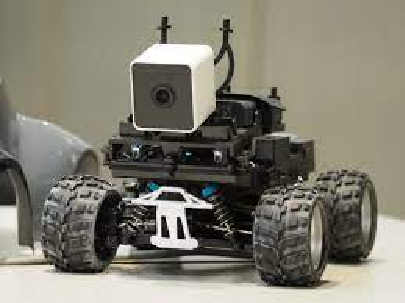
\includegraphics[width=\textwidth]{Imagenes/IA/deepracer.pdf}
    \caption{Vehículo Amazon DeepRacer utilizado}
    \label{deepracer}
\end{figure}

Gracias a que nuestra escuela, ETSIT de la Universidad de Valladolid, poseía un pequeño circuito para trabajar con el vehículo, lo montamos y dispusimos varias señales de tráfico a lo largo de la maqueta. Así, pudimos probar el rendimiento de nuestro algoritmo de detección y los pesos de entrenamiento que posee. Tal y como podemos observar en las figuras \ref{deteccion1} y \ref{deteccion2}, logramos la detección de las señales a lo largo de la maqueta, a pesar de la calidad del vídeo y de que las señales miniatura no sean exactamente igual a las reales. \\

\begin{figure}[H]
    \centering
 	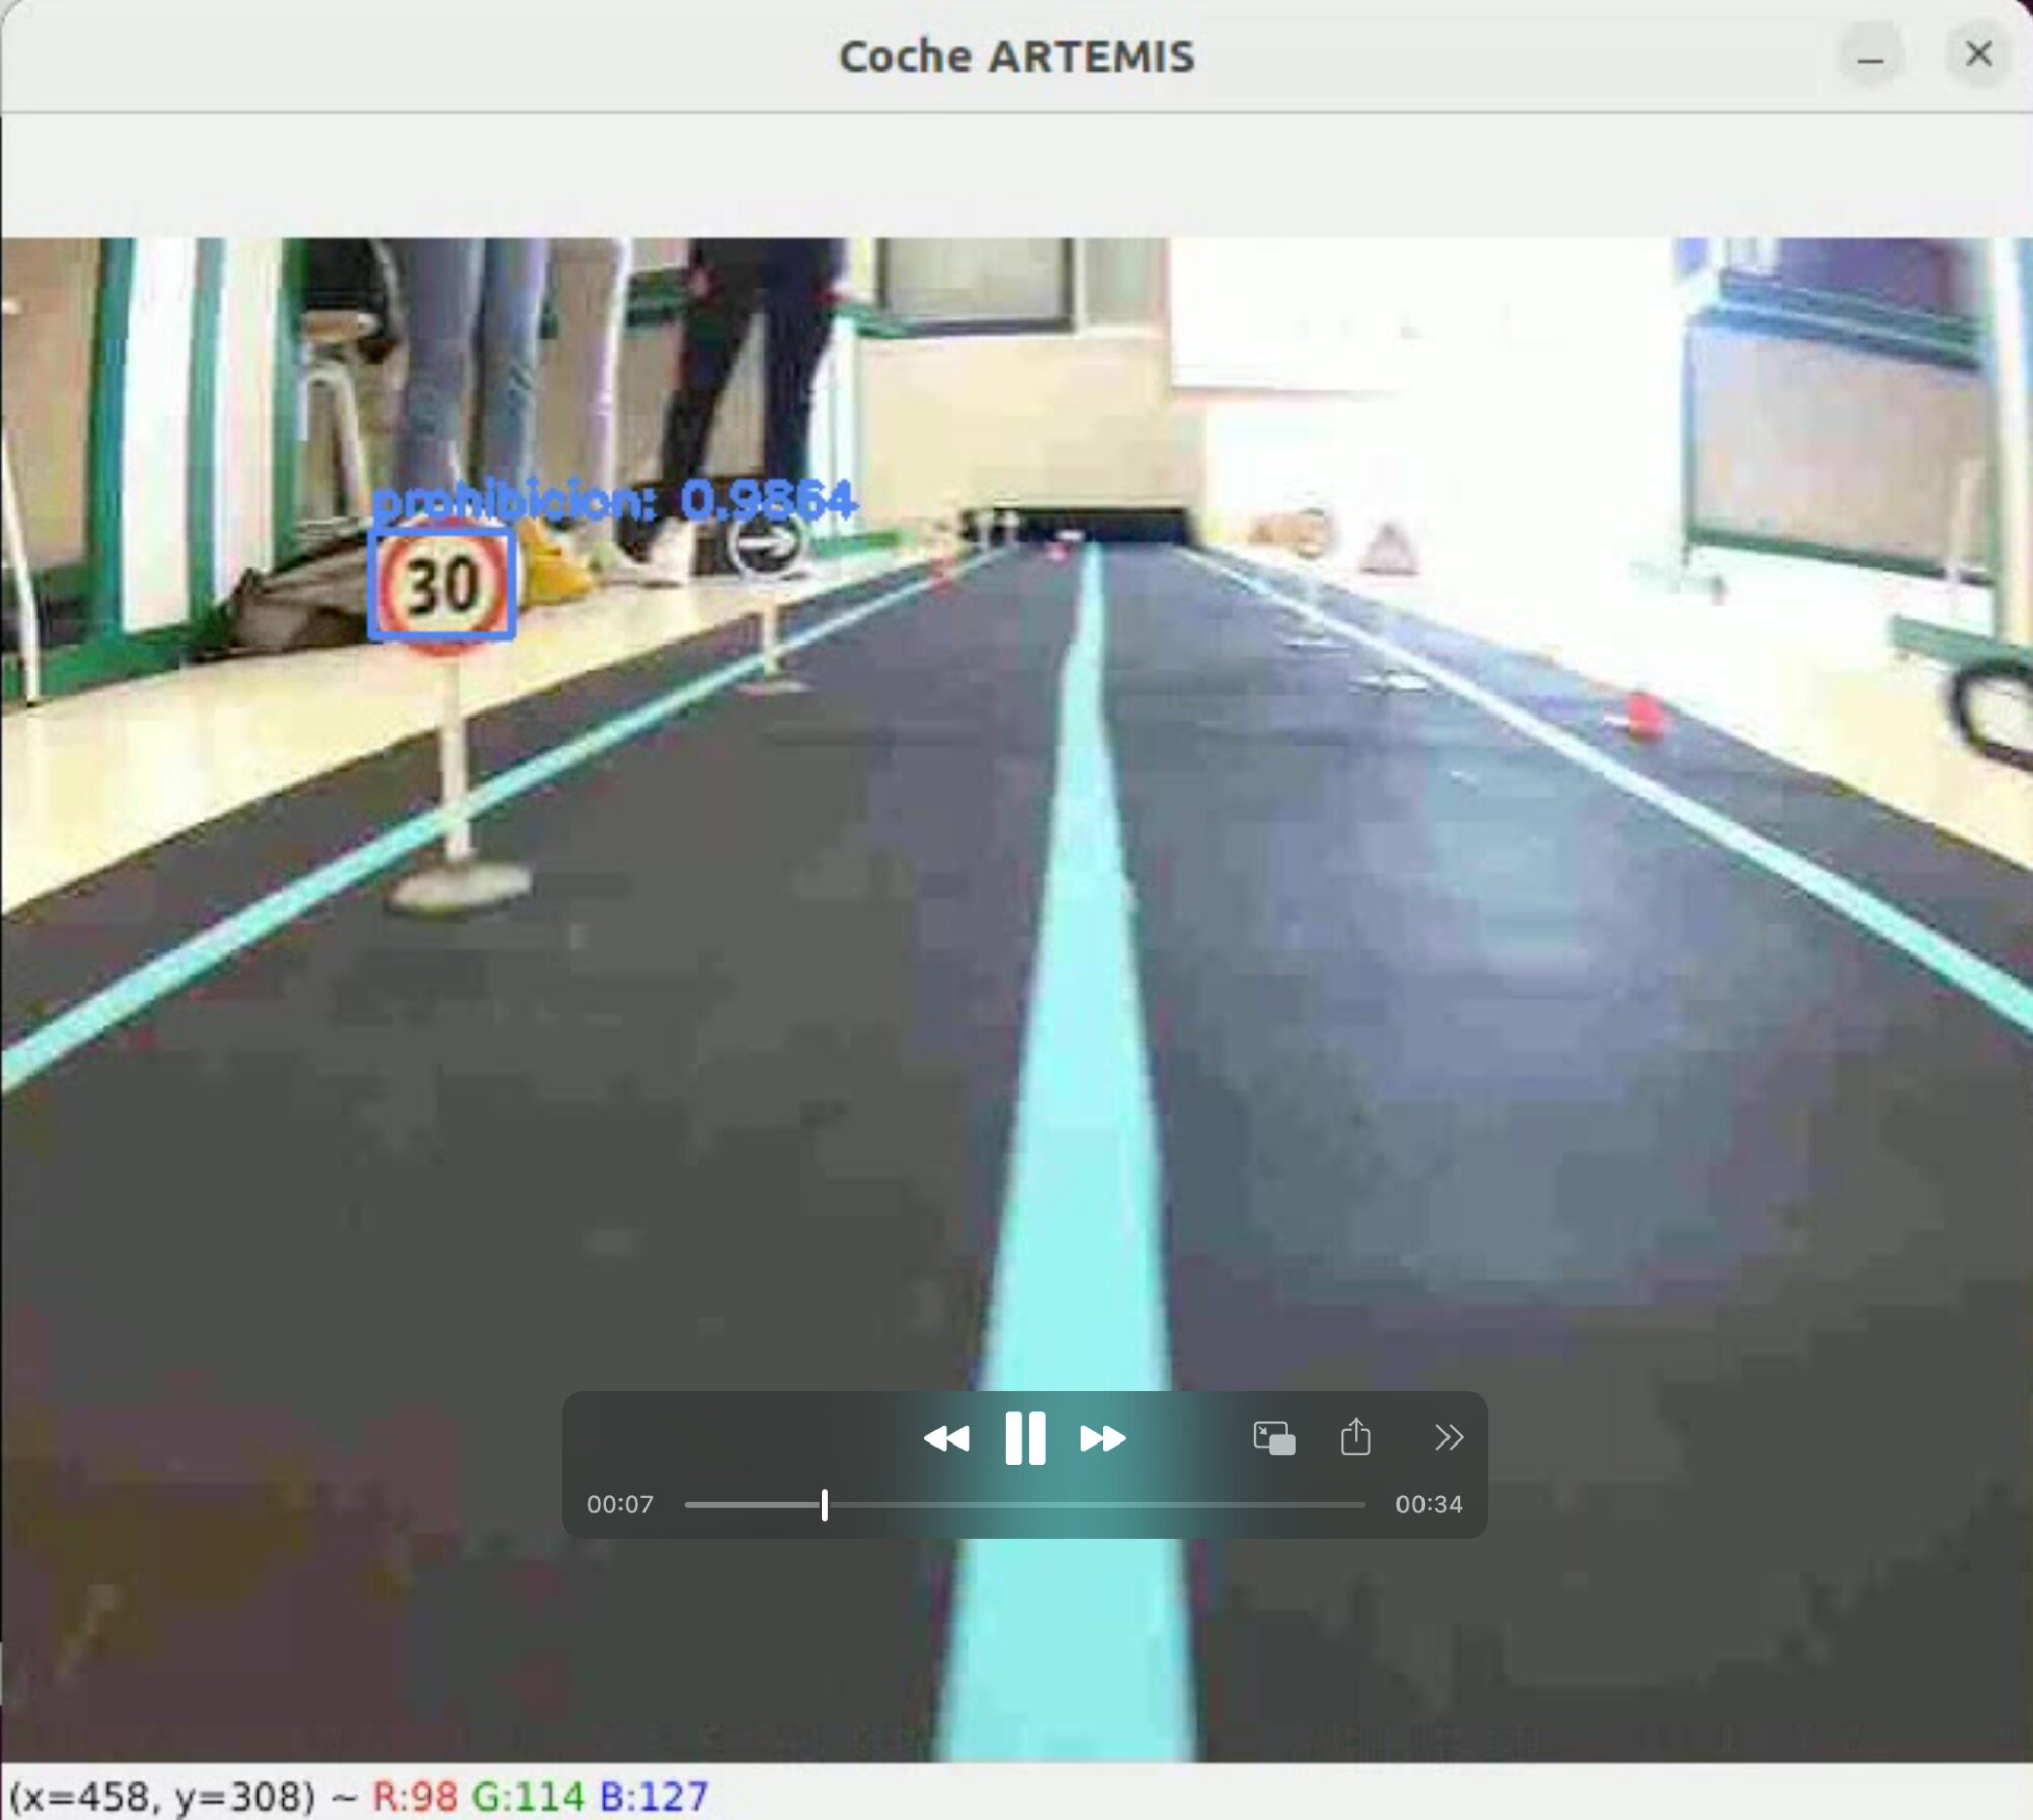
\includegraphics[width=\textwidth]{Imagenes/IA/deteccion1.pdf}
    \caption{Primer ejemplo de detección de señales miniatura en vídeo en circuito}
    \label{deteccion1}
\end{figure}

\begin{figure}[H]
    \centering
 	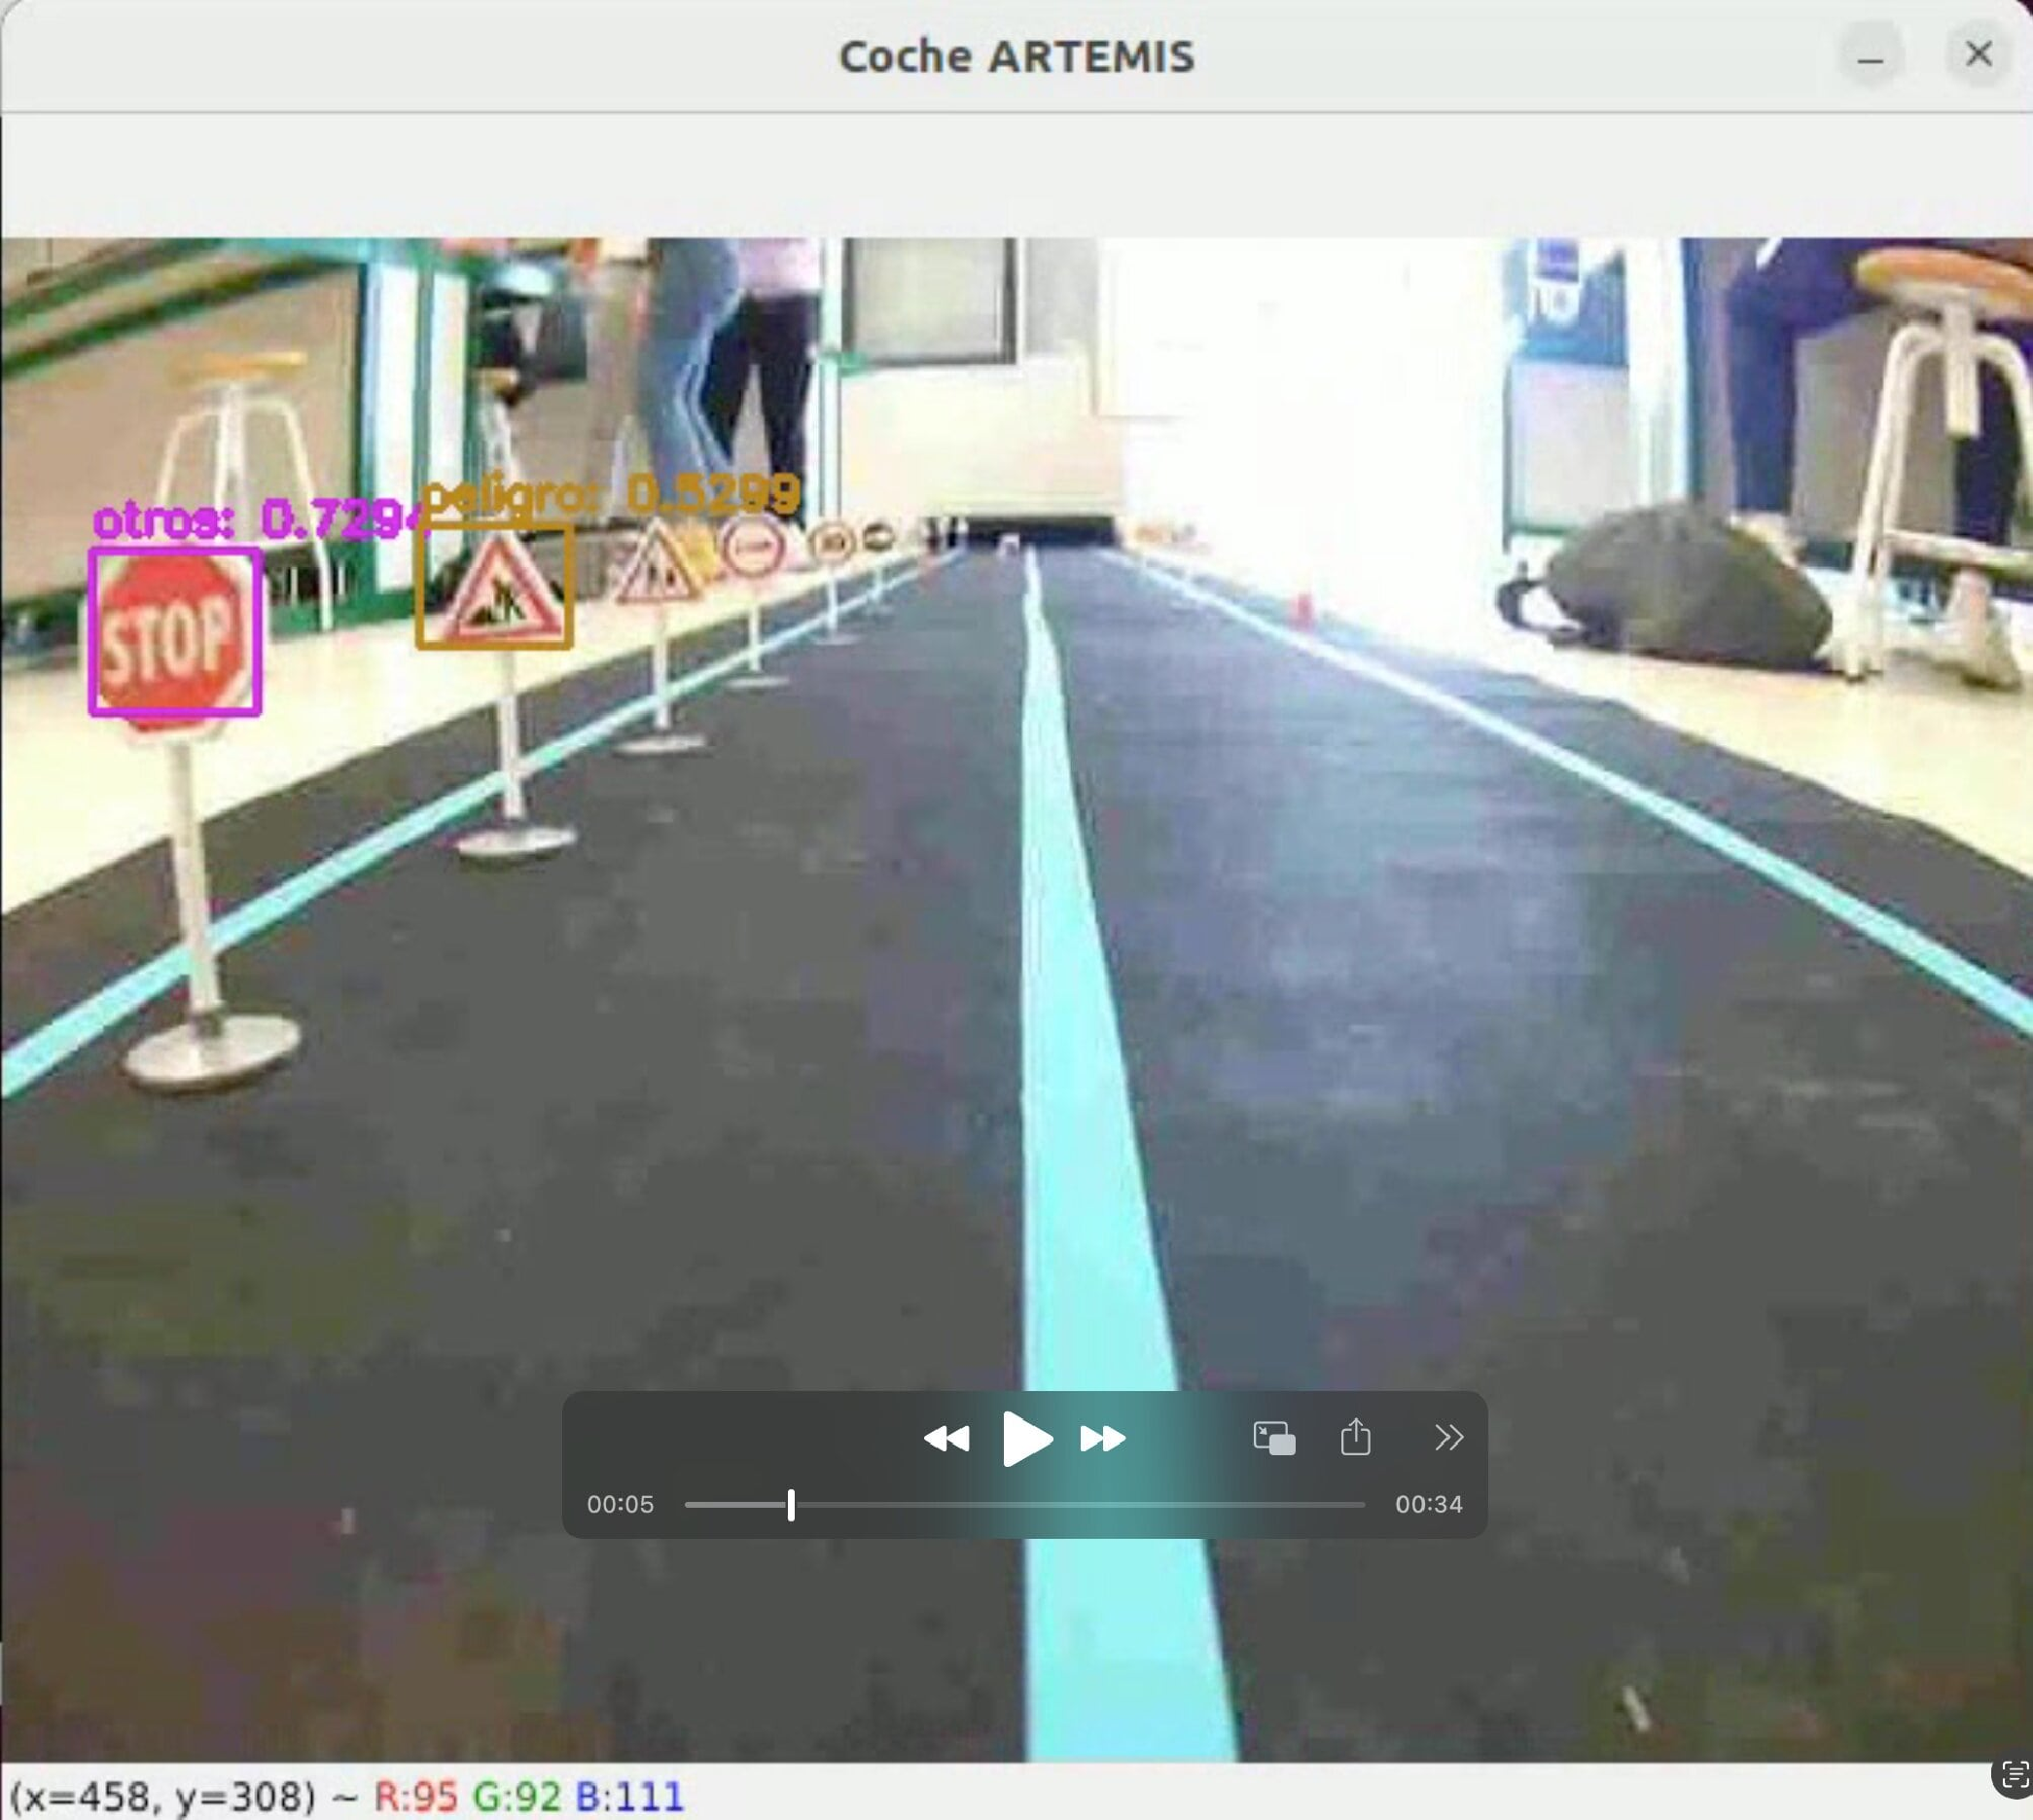
\includegraphics[width=\textwidth]{Imagenes/IA/deteccion2.pdf}
    \caption{Segundo ejemplo de detección de señales miniatura en vídeo en circuito}
    \label{deteccion2}
\end{figure}

De igual forma, podemos probar con imágenes de una vía normal, podemos visualizar el procesado de nuestro algoritmo en la figura \ref{deteccion3}\\

\begin{figure}[H]
    \centering
 	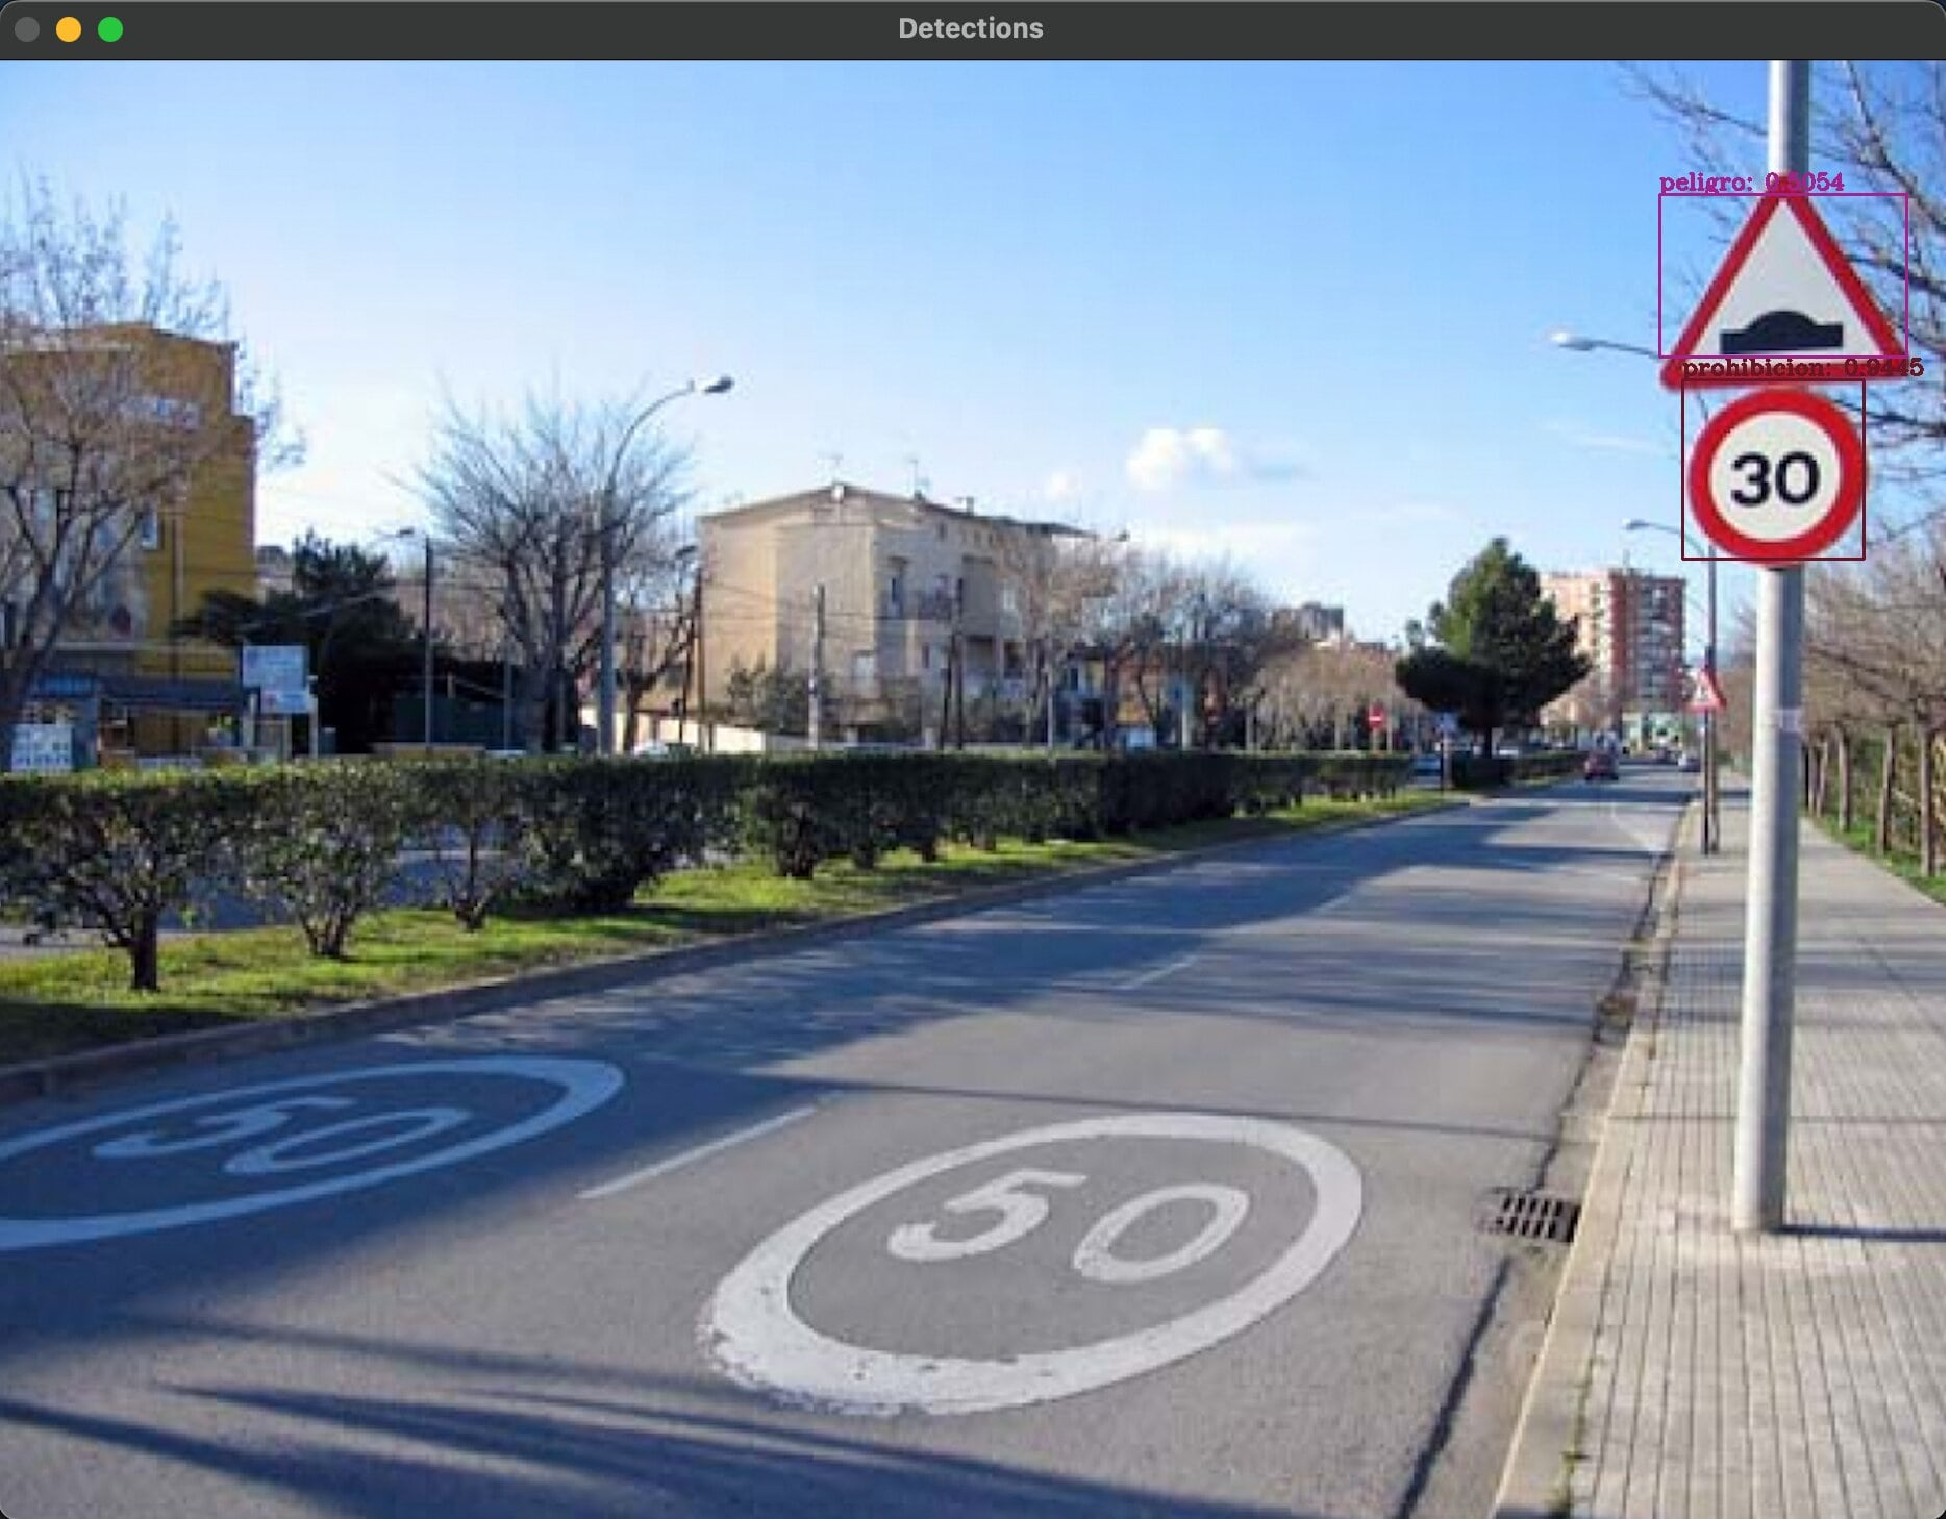
\includegraphics[width=\textwidth]{Imagenes/IA/deteccion3.pdf}
    \caption{Detección de señales reales en vídeo en carretera real}
    \label{deteccion3}
\end{figure}

Finalmente, a través de un popular repositorio de GitHub \url{https://github.com/rafaelpadilla/Object-De\ tection-Metrics.git} dedicado a medir el rendimiento de algoritmos de detección, podremos analizar nuestro sistema de detección de señales. A través de 64 imágenes etiquetadas y procesadas por el algoritmo, podremos medir el rendimiento de la red mediante sus detecciones. En concreto, podremos obtener la curva de Precisión vs Recuperación (Precision vs Recall) de nuestro modelo. La precisión es un término que describe la medida verdaderos positivos (TP) en relación con los falsos positivos (FP). Por otro lado, la recuperación se refiere a la proporción de verdaderos positivos (TP) en comparación con la suma de verdaderos positivos y falsos negativos (FN). En resumen, estos conceptos son utilizados para evaluar la efectividad de un modelo de clasificación y se pueden emplear para establecer el límite óptimo del modelo.\\

Para calcular la precisión y la recuperación se hace uso de las siguientes fórmulas:\\
\\
$$\text{precisión} = \frac{\text{TP}}{\text{TP} + \text{FP}}\ \text{recuperación} = \frac{\text{TP}}{\text{TP} + \text{FN}}$$
\\

Podemos contemplar en la figura XXX (rendimiento.pdf) que para cada categoría contemplada de señales de tráfico obtenemos una precisión media (AP) diferente. Para la clase obligación se obtiene una precisión del 57,9\%, para peligro un 72,22\%, para prohibición un 84,54\% y para el resto un 62,14\%. Destacar que entre las 64 imágenes que se han analizado, se encontraban tanto imágenes de señales reales, como señales de juguete, esto es clave porque los pesos pre-entrenados no contaban con señales falsas. Por ello, podemos notar que quizás los valores de precisión obtenidos no son suficientemente altos debido a la inclusión de señales que no se asemejan con las de entrenamiento.\\


\begin{figure}[H]
    \centering
 	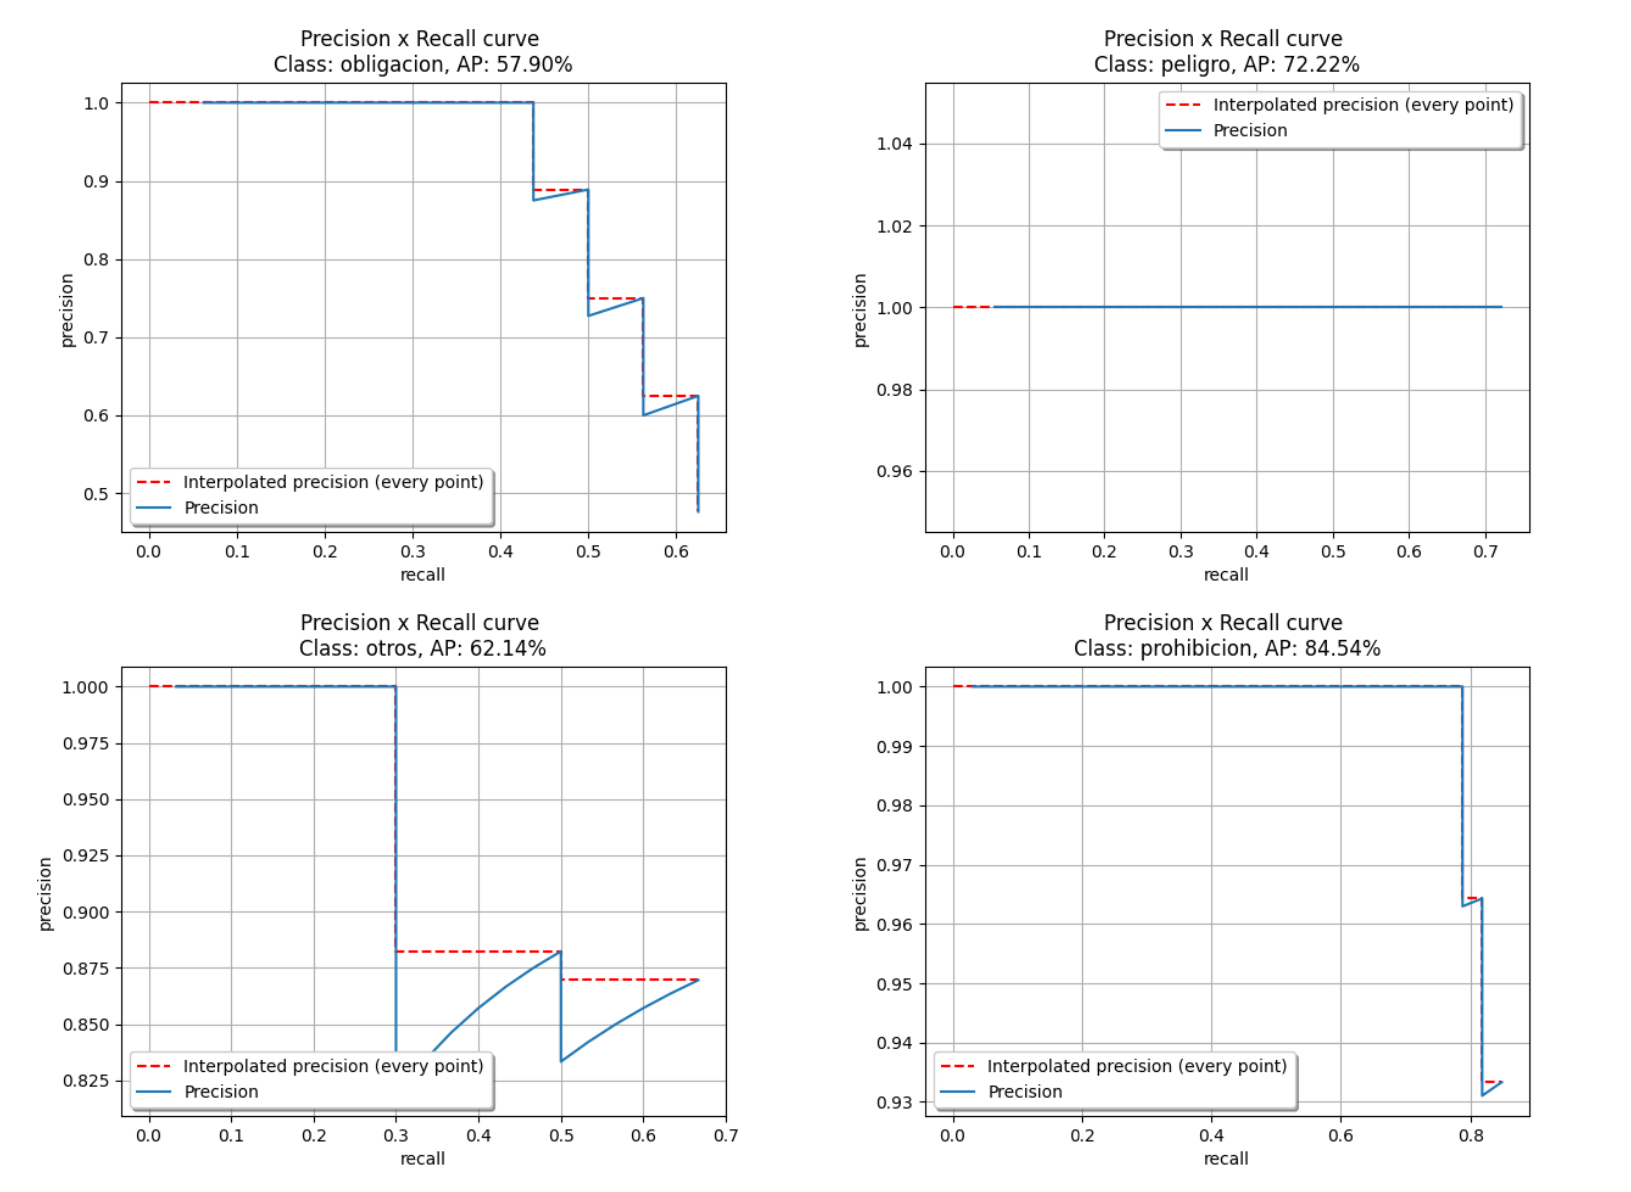
\includegraphics[width=\textwidth]{Imagenes/IA/rendimiento.pdf}
    \caption{Gráficas del rendimiento obtenido}
    \label{rendimiento}
\end{figure}